% =====================================================================
% Semana 1 · S1.3 — Paralelo, KCL y resistencia equivalente
% Fundamentos de Sistemas Electrónicos Analógicos (Ingeniería Aeroespacial)
% Compilar: pdflatex semana_1_s13_paralelo_kcl.tex  (2 pasadas)
% =====================================================================
\documentclass[aspectratio=169]{beamer}

\usepackage[utf8]{inputenc}
\usepackage[T1]{fontenc}
\usepackage{lmodern}
\usepackage[spanish,es-tabla]{babel}
\usepackage{amsmath,amssymb}
\usepackage{siunitx}
\usepackage{booktabs}
\usepackage{microtype}
\usepackage{circuitikz}

% ---- Paleta del curso (navy/gold) ------------------------------------
\definecolor{navy}{RGB}{23,54,93}       % 17365D
\definecolor{navysoft}{RGB}{72,101,140}
\definecolor{gold}{RGB}{179,142,62}     % B38E3E
\definecolor{ink}{RGB}{44,51,58}
\definecolor{soft}{RGB}{244,241,234}    % F4F1EA

\usetheme{default}
\setbeamertemplate{navigation symbols}{}
\setbeamertemplate{footline}[frame number]
\setbeamercolor{structure}{fg=navy}
\setbeamercolor{frametitle}{fg=white,bg=navy}
\setbeamercolor{title}{fg=navy}
\setbeamercolor{subtitle}{fg=navysoft}
\setbeamercolor{itemize item}{fg=gold}
\setbeamercolor{itemize subitem}{fg=gold}
\setbeamercolor{block title}{fg=white,bg=navy}
\setbeamercolor{block body}{bg=soft}
\setbeamercolor{example text}{fg=navy}
\setbeamertemplate{itemize item}{\scriptsize\raise1.25pt\hbox{\donotcoloroutermaths$\bullet$}}
\setbeamertemplate{itemize subitem}{\scriptsize\raise1.25pt\hbox{\donotcoloroutermaths$\circ$}}
\setbeamerfont{frametitle}{size=\large,series=\bfseries}

\title[Paralelo y KCL]{Paralelo, KCL y resistencia equivalente}
\subtitle{S1.3 — Simulaciones y laboratorio de la Semana 1}
\institute{Licenciatura en Ingeniería Aeroespacial\\ UNAM · ENES Unidad Juriquilla}
\author{M. en C. José de Jesús Santana Ramírez}
\date{Semestre 2027-1}

\begin{document}

% ---------------------------------------------------------------------
\begin{frame}[plain]
  \titlepage
\end{frame}

% ---------------------------------------------------------------------
\begin{frame}{Objetivos de la sesión}
  \begin{itemize}
    \item Definir una conexión \textbf{en paralelo} y sus propiedades inmediatas.
    \item Usar la \textbf{conductancia} $G = 1/R$ para sumar ramas en paralelo.
    \item Calcular la \textbf{resistencia equivalente} y verificar que $R_{eq} < R_{mín}$.
    \item Aplicar la \textbf{Ley de corrientes de Kirchhoff (KCL)} en el nodo del bus y en el retorno.
    \item Desarrollar por completo el ejercicio del bus de \SI{5}{\volt} con
      $1\,\text{k}\Omega$, $2.2\,\text{k}\Omega$ y $3.3\,\text{k}\Omega$.
  \end{itemize}
  \pause
  \begin{block}{Pregunta inicial}
    ¿Qué rama conduce más corriente y por qué?
  \end{block}
\end{frame}

% ---------------------------------------------------------------------
\begin{frame}{Teoría 1 · ¿Qué es una conexión en paralelo?}
  Dos o más elementos están \textbf{en paralelo} cuando comparten el \textbf{mismo
  par de nodos}: todos ven la misma tensión y la corriente de la fuente se reparte.

  \begin{columns}[T]
    \begin{column}{0.5\textwidth}
      \resizebox{0.95\linewidth}{!}{%
      \begin{circuitikz}[american voltages, scale=0.95]
        \draw (0,3) to[V, l=$V_{bus}$, i=$I$] (0,0);
        \draw (0,3) -- (8,3);
        \draw (0,0) -- (8,0);
        \draw (2,3) to[R, l=$R_1$] (2,0);
        \draw (4.2,3) to[R, l=$R_2$] (4.2,0);
        \draw (6.4,3) to[R, l=$R_3$] (6.4,0);
      \node[ground] at (0,0) {};
      \end{circuitikz}}
    \end{column}
    \begin{column}{0.45\textwidth}
      \begin{itemize}
        \item Tensión común: $V_{R1} = V_{R2} = V_{R3} = V_{bus}$.
        \item Cada rama conduce $I_k = V_{bus}/R_k$.
        \item La corriente total es la \textbf{suma} de ramas (KCL).
        \item $R_{eq}$ es \textbf{menor} que la rama de menor valor.
      \end{itemize}
    \end{column}
  \end{columns}
\end{frame}

% ---------------------------------------------------------------------
\begin{frame}{Teoría 2 · Conductancia y resistencia equivalente}
  \begin{block}{Conductancia}
    $G = \dfrac{1}{R}$ \ (siemens, S): mide cuánta corriente deja pasar un
    elemento por cada voltio aplicado. En paralelo las conductancias \textbf{se suman}:
  \end{block}
  \[
    G_t = G_1 + G_2 + G_3 = \frac{1}{R_1} + \frac{1}{R_2} + \frac{1}{R_3}
    \qquad\qquad
    R_{eq} = \frac{1}{G_t}
  \]
  \pause
  \begin{itemize}
    \item Dos resistencias: $R_{eq} = \dfrac{R_1\cdot R_2}{R_1 + R_2}$ (solo para dos).
    \item \textbf{Reglas de verificación:} $R_{eq} < R_{mín}$; si todas son $R$, $R_{eq} = R/n$.
    \item $G$ es la pendiente de $I$ vs $V$ de cada rama: conecta con la pendiente-conductancia de S1.1.
  \end{itemize}
\end{frame}

% ---------------------------------------------------------------------
\begin{frame}{Teoría 3 · Ley de corrientes de Kirchhoff (KCL)}
  \begin{block}{Enunciado}
    En cualquier \textbf{nodo}, la suma de las corrientes que \textbf{entran} es
    igual a la suma de las que \textbf{salen}: $\displaystyle\sum I_{nodo} = 0$.
  \end{block}
  \pause
  En el nodo superior (bus):
  \[
    I_{fuente} = I_{R1} + I_{R2} + I_{R3}
  \]
  \pause
  \begin{itemize}
    \item La KCL también se cumple en el \textbf{nodo de retorno}: la corriente
      que regresa por tierra es exactamente la suma de ramas.
    \item Si ``falta'' corriente en un nodo: fuga, rama no contada o error de medición.
  \end{itemize}
\end{frame}

% ---------------------------------------------------------------------
\begin{frame}{Teoría 4 · Divisor de corriente}
  La corriente de cada rama es proporcional a su conductancia:
  \[
    I_k = I_{fuente}\cdot\frac{G_k}{G_t} = I_{fuente}\cdot\frac{R_{eq}}{R_k}
  \]
  \pause
  \begin{itemize}
    \item \textbf{La rama de menor resistencia (mayor conductancia) conduce la
      mayor corriente.} (Respuesta a la pregunta inicial.)
    \item En paralelo, la corriente se reparte en proporción inversa a la resistencia.
    \item Análogo del divisor de tensión, pero para corrientes.
  \end{itemize}
\end{frame}

% ---------------------------------------------------------------------
\begin{frame}{Teoría 5 · Balance de potencia en paralelo}
  La misma conservación de la energía de S1.2:
  \[
    \boxed{\;P_{fuente}\ (\text{entregada}) = V_{bus}\cdot I_{fuente}
      = P_1 + P_2 + P_3 = V_{bus}^2\,(G_1 + G_2 + G_3)\;}
  \]
  \pause
  \begin{itemize}
    \item Cada rama disipa $P_k = V_{bus}^2/R_k$.
    \item \textbf{Contraste con serie:} aquí la rama de \emph{menor} resistencia
      disipa \emph{más} potencia.
  \end{itemize}
\end{frame}

% ---------------------------------------------------------------------
\begin{frame}{Ejercicio · Enunciado}
  \begin{block}{Bus en paralelo de la simulación S1.3}
    \centering
    $V_{bus} = \SI{5}{\volt}$, \quad $R_1 = \SI{1}{\kilo\ohm}$,
    $R_2 = \SI{2.2}{\kilo\ohm}$, \quad $R_3 = \SI{3.3}{\kilo\ohm}$.
  \end{block}
  \begin{center}
    \begin{circuitikz}[american voltages, scale=0.95]
      \draw (0,3) to[V, l={$V_{bus}=5\,\mathrm{V}$}, i=$I$] (0,0);
      \draw (0,3) -- (8.6,3);
      \draw (0,0) -- (8.6,0);
      \draw (2.4,3) to[R, l=$R_1$] (2.4,0);
      \draw (4.8,3) to[R, l=$R_2$] (4.8,0);
      \draw (7.2,3) to[R, l=$R_3$] (7.2,0);
    \node[ground] at (0,0) {};
    \end{circuitikz}
  \end{center}
  \textbf{Determinar:} $G_1$, $G_2$, $G_3$, $G_t$, $R_{eq}$, $I_1$, $I_2$, $I_3$,
  $I_{fuente}$, $P_1$, $P_2$, $P_3$, y verificar KCL y balance de potencia.
\end{frame}

% ---------------------------------------------------------------------
\begin{frame}{Desarrollo del ejercicio · Paso 1 — Conductancias}
  \[
    G_1 = \frac{1}{1\,\text{k}\Omega} = \SI{1.000}{\milli\siemens}
    \qquad
    G_2 = \frac{1}{2.2\,\text{k}\Omega} = \SI{0.4545}{\milli\siemens}
    \qquad
    G_3 = \frac{1}{3.3\,\text{k}\Omega} = \SI{0.3030}{\milli\siemens}
  \]
  \pause
  \begin{itemize}
    \item \textbf{Predicción:} la rama de menor resistencia ($R_1$) tendrá la mayor
      conductancia y, por tanto, la mayor corriente.
    \item Unidad: siemens (S); en mili: \SI{1}{\milli\siemens} = \num{e-3} S.
  \end{itemize}
\end{frame}

% ---------------------------------------------------------------------
\begin{frame}{Desarrollo del ejercicio · Paso 2 — Conductancia total y $R_{eq}$}
  \[
    G_t = G_1 + G_2 + G_3 = (1.000 + 0.4545 + 0.3030)\ \text{mS}
        = \SI{1.7576}{\milli\siemens}
  \]
  \[
    R_{eq} = \frac{1}{G_t} = \frac{1}{1.7576\times 10^{-3}\ \text{S}}
    = \SI{568.97}{\ohm}
  \]
  \pause
  \begin{block}{Verificación}
    $R_{eq} = 568.97\ \Omega < R_{mín} = 1\,\text{k}\Omega$ \checkmark
    (más ramas en paralelo $\Rightarrow$ menos resistencia vista por la fuente).
  \end{block}
\end{frame}

% ---------------------------------------------------------------------
\begin{frame}{Desarrollo del ejercicio · Paso 3 — Corrientes de rama}
  \begin{align*}
    I_1 &= \frac{V_{bus}}{R_1} = \frac{\SI{5}{\volt}}{\SI{1}{\kilo\ohm}}
           = \SI{5.000}{\milli\ampere}\\[2pt]
    I_2 &= \frac{V_{bus}}{R_2} = \frac{\SI{5}{\volt}}{\SI{2.2}{\kilo\ohm}}
           = \SI{2.273}{\milli\ampere}\\[2pt]
    I_3 &= \frac{V_{bus}}{R_3} = \frac{\SI{5}{\volt}}{\SI{3.3}{\kilo\ohm}}
           = \SI{1.515}{\milli\ampere}
  \end{align*}
  \pause
  \begin{itemize}
    \item Confirmado: $I_1 > I_2 > I_3$ (la menor resistencia, mayor corriente).
    \item O bien con el divisor: $I_k = I_{fuente}\cdot R_{eq}/R_k$.
  \end{itemize}
\end{frame}

% ---------------------------------------------------------------------
\begin{frame}{Desarrollo del ejercicio · Paso 4 — KCL (corriente de fuente)}
  \[
    I_{fuente} = I_1 + I_2 + I_3
    = \SI{5.000}{\milli\ampere} + \SI{2.273}{\milli\ampere} + \SI{1.515}{\milli\ampere}
  \]
  \[
    \boxed{\;I_{fuente} = \SI{8.788}{\milli\ampere}\;}
  \]
  \pause
  \begin{itemize}
    \item Verificación cruzada: $I_{fuente} = V_{bus}/R_{eq} = 5/568.97 =
      \SI{8.788}{\milli\ampere}$ \checkmark
    \item La misma suma debe aparecer en el \textbf{nodo de retorno} (tierra).
  \end{itemize}
\end{frame}

% ---------------------------------------------------------------------
\begin{frame}{Desarrollo del ejercicio · Paso 5 — Potencias}
  \begin{align*}
    P_1 &= \frac{V_{bus}^2}{R_1} = \frac{25}{1\,\text{k}\Omega} = \SI{25.00}{\milli\watt}\\[2pt]
    P_2 &= \frac{V_{bus}^2}{R_2} = \frac{25}{2.2\,\text{k}\Omega} = \SI{11.36}{\milli\watt}\\[2pt]
    P_3 &= \frac{V_{bus}^2}{R_3} = \frac{25}{3.3\,\text{k}\Omega} = \SI{7.58}{\milli\watt}
  \end{align*}
  \pause
  \begin{itemize}
    \item \textbf{En paralelo, $P \propto 1/R$}: la rama de menor resistencia
      disipa más ($P_1 > P_2 > P_3$) — contraste con la serie.
  \end{itemize}
\end{frame}

% ---------------------------------------------------------------------
\begin{frame}{Desarrollo del ejercicio · Paso 6 — Balance de potencia}
  \begin{align*}
    \sum P &= P_1 + P_2 + P_3
             = \SI{25.00}{\milli\watt} + \SI{11.36}{\milli\watt} + \SI{7.58}{\milli\watt}
             = \SI{43.94}{\milli\watt}\\[4pt]
    P_{fuente} &= V_{bus}\cdot I_{fuente}
                 = \SI{5}{\volt}\cdot \SI{8.788}{\milli\ampere}
                 = \SI{43.94}{\milli\watt}
  \end{align*}
  \[
    \boxed{\;P_{fuente} = \sum P \qquad\checkmark\;}
  \]
  \pause
  \begin{itemize}
    \item La fuente entrega exactamente lo que disipan las tres ramas.
    \item En LTspice: $V(bus)\cdot I(V1)$ negativo; el balance suma con signo.
  \end{itemize}
\end{frame}

% ---------------------------------------------------------------------
\begin{frame}{Desarrollo del ejercicio · Paso 7 — Derating}
  \begin{itemize}
    \item Límite con derating de 50\,\%: $P_{derated} = \SI{125}{\milli\watt}$.
    \item Peor caso de la red: $P_1 = \SI{25.00}{\milli\watt}$ (rama de $1\,\text{k}\Omega$).
  \end{itemize}
  \[
    \text{margen} = \frac{125}{25.0} = 5\times
  \]
  \begin{block}{Decisión de diseño}
    El peor caso usa 20\,\% del límite con derating $\rightarrow$ \textbf{aceptado
    con margen}. Si el bus subiera a 12 V, $P_1 = 144$ mW y esta rama ya excedería
    el límite (misma advertencia que en S1.1).
  \end{block}
\end{frame}

% ---------------------------------------------------------------------
\begin{frame}[fragile]{Verificación en LTspice}
  Abrir \texttt{semana1\_03\_kcl\_paralelo.asc}, ejecutar \texttt{.op} y consultar
  \texttt{View > SPICE Error Log}. El esquema ya mide las tres corrientes de rama,
  la corriente de fuente y el error de KCL; para cerrar el balance agregar:

  \begin{verbatim}
.meas op P_R1_mW PARAM V(bus)*V(bus)/1k*1e3
.meas op P_R2_mW PARAM V(bus)*V(bus)/2.2k*1e3
.meas op P_R3_mW PARAM V(bus)*V(bus)/3.3k*1e3
.meas op P_fuente_mW PARAM V(bus)*(-I(V1))*1e3
.meas op Balance_mW PARAM P_fuente_mW-(P_R1_mW+P_R2_mW+P_R3_mW)
  \end{verbatim}

  \textbf{Criterio de éxito:} \texttt{KCL\_error\_uA} $\approx 0$ y
  \texttt{Balance\_mW} $\approx 0$.
\end{frame}

% ---------------------------------------------------------------------
\begin{frame}{Resultado de la simulación}
  \begin{center}
    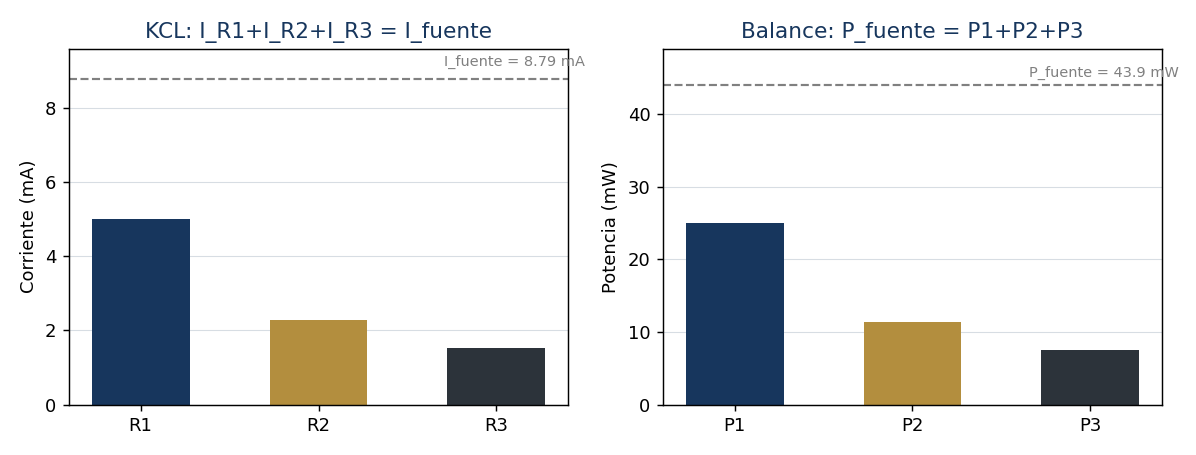
\includegraphics[width=0.82\textwidth]{figs/s13_kcl_balance.png}
  \end{center}
  \begin{itemize}
    \item \textbf{KCL:} $I_{R1}+I_{R2}+I_{R3} = 8.79\,\text{mA} = I_{fuente}$: la suma de las corrientes de rama.
    \item \textbf{Balance de potencia:} $P_{fuente} = 43.9\,\text{mW} = P_1+P_2+P_3$: la energía se conserva.
    \item \textbf{La rama de menor resistencia ($R_1 = 1\,\text{k}\Omega$) lleva más corriente y disipa más}: en paralelo, $P \propto 1/R$.
  \end{itemize}
\end{frame}

% ---------------------------------------------------------------------
\begin{frame}{Errores comunes}
  \begin{table}
    \small
    \begin{tabular}{p{0.34\textwidth}p{0.28\textwidth}p{0.32\textwidth}}
      \toprule
      Error & Consecuencia & Corrección \\
      \midrule
      Sumar resistencias en paralelo como serie & $R_{eq}$ demasiado grande & Sumar conductancias: $1/R_{eq} = \sum 1/R$ \\
      Usar $(R_1R_2)/(R_1+R_2)$ con tres ramas & $R_{eq}$ incorrecta & Esa fórmula solo vale para dos \\
      Creer que la mayor $R$ lleva más corriente & Orden invertido & $I_k \propto 1/R_k$ \\
      Olvidar que $R_{eq} < R_{mín}$ & No detectar el error & Verificación rápida siempre \\
      Calcular $P_k$ con la corriente total & Potencias $\approx 3\times$ mayores & Cada rama usa su propia corriente \\
      \bottomrule
    \end{tabular}
  \end{table}
\end{frame}

% ---------------------------------------------------------------------
\begin{frame}{Lectura aeroespacial}
  \begin{itemize}
    \item \textbf{Dimensionar la fuente por la suma:} el bus de aviónica alimenta
      cargas en paralelo; la fuente y su protección se dimensionan con $\sum I_k$
      en el peor caso, no con la carga ``típica''. Es el mismo criterio del EPS:
      $P_{bus} = V_{bus}\cdot\sum I_k$.
    \item \textbf{Protección por rama:} cada rama lleva su fusible; si una carga
      falla en corto, su protección debe abrir \emph{antes} de tumbar el bus
      (KCL explica por qué un corto en una rama dispara todo sin aislamiento).
    \item \textbf{Redundancia en paralelo:} calefactores o sensores redundantes:
      si una rama se abre, las demás mantienen tensión y corriente (la fuente
      entrega menos). Topología natural para tolerancia a fallas.
    \item \textbf{Retorno de tierra:} la KCL del nodo de retorno justifica el
      \emph{single-point ground}: corrientes de retorno por caminos distintos
      crean diferencias de potencial entre ``tierras'' (ruido de masa).
    \item \textbf{Celdas solares:} en paralelo suman corriente a tensión
      constante; en serie suman tensión. El panel combina ambas.
  \end{itemize}
\end{frame}

% ---------------------------------------------------------------------
\begin{frame}{Preguntas de verificación}
  \begin{enumerate}
    \item ¿Por qué la rama de $1\,\text{k}\Omega$ conduce más corriente que la de $3.3\,\text{k}\Omega$?
    \item Si se abre la rama de $1\,\text{k}\Omega$, ¿qué pasa con las otras dos ramas y con la fuente?
      \uncover<2->{\emph{(Las ramas no cambian; la fuente entrega menos.)}}
    \item ¿Cómo cambia $R_{eq}$ si se agrega una cuarta rama de $10\,\text{k}\Omega$?
      \uncover<3->{\emph{(Baja: más conductancia en paralelo.)}}
    \item Con $V_{bus} = \SI{5}{\volt}$, ¿cuánto disipa la rama de $2.2\,\text{k}\Omega$?
      \uncover<4->{\emph{(\SI{11.36}{\milli\watt}.)}}
    \item ¿Por qué un fusible por rama protege mejor el bus que un solo fusible general?
  \end{enumerate}
\end{frame}


\end{document}
